\documentclass[12pt,a4paper]{article}
\usepackage{amsmath, amssymb, geometry, booktabs, xcolor, hyperref,
            listings, pgfplots, tcolorbox, enumitem, fancyhdr, tikz, array}
\usepgfplotslibrary{fillbetween}
\geometry{margin=2.5cm}
\pgfplotsset{compat=1.18}
\tcbuselibrary{skins, breakable}

% Define custom environments
\newtcolorbox{curiositybox}[1]{colback=yellow!10, colframe=orange!80, title=#1, breakable}
\newtcolorbox{infobox}[1]{colback=blue!5, colframe=blue!60, title=#1, breakable}
\newtcolorbox{mistakebox}[1]{colback=red!5, colframe=red!60, title=#1, breakable}
\newtcolorbox{learnbox}[1]{colback=green!5, colframe=green!60, title=#1, breakable}

% Header and Footer
\pagestyle{fancy}
\fancyhf{}
\lhead{Applications of Multiple Integration}
\rhead{Unit 5 --- LAC}
\cfoot{\thepage}

% Document Title Setup
\title{\textbf{Applications of Multiple Integration} \\ \large Unit 5: Multiple Integrals and Coordinate Transformations}
\author{Department of Mathematics}
\date{\today}

\begin{document}
\maketitle
\tableofcontents
\newpage

%=============================================================
\section{Real-World Engineering Hook}
%=============================================================

\begin{curiositybox}{Why Should an Engineer Care?}
Imagine you are a civil engineer designing a curved concrete dam. Water presses against the entire submerged face with a force that varies with depth --- the deeper the point, the higher the pressure. To find the \emph{total} force, you cannot just multiply pressure by area, because the pressure is not uniform. You must integrate the pressure function over the entire curved surface using a double integral.

Now picture a mechanical engineer who must verify that a complex turbine casting rotates smoothly at 3000~rpm. If the centre of gravity is even a few millimetres off-axis, the imbalance generates vibrations that crack bearings within hours. Finding the exact centroid requires computing the mass and first moments as double integrals over the casting cross-section.

Finally, consider an electrical engineer depositing charge on a silicon wafer where the surface charge density \(\sigma(x,y)\) varies across the chip. The total charge --- critical for device calibration --- is \(Q = \iint_R \sigma(x,y)\,dA\). Every one of these engineering quantities, from fluid pressure to rotating-mass balance to charge deposition, reduces to setting up and evaluating a multiple integral with the correct physical density function.
\end{curiositybox}

%=============================================================
\section{Why This Topic Exists}
%=============================================================

\begin{center}
\begin{tabular}{>{\bfseries}p{6cm} p{8cm}}
\toprule
Theoretical Concept & Engineering Application / Consequence of Misunderstanding \\
\midrule
Area and volume by double/triple integrals &
Structural cross-section properties; tank and reservoir capacity design. An error in computed volume means incorrect material quantities and potential structural failure. \\[6pt]
Mass and centroid &
Balancing rotating machinery; locating neutral axes in beams. A wrong centroid shifts the axis of rotation, inducing vibration, fatigue, and early mechanical failure. \\[6pt]
Moment of inertia &
Beam bending resistance and flywheel energy storage. Under-estimating \(I\) leads to beams that deflect beyond permissible limits or collapse under design loads. \\[6pt]
Engineering application integrals &
Fluid pressure on gates and dams, charge distribution on wafers, probability from joint density functions --- all are direct design inputs that drive safety factors and device specifications. \\
\bottomrule
\end{tabular}
\end{center}

\begin{learnbox}{Core Objective}
After studying this topic you will be able to set up and evaluate double and triple integrals to compute areas, volumes, masses, centroids, moments of inertia, and real engineering quantities such as fluid pressure and electric charge. You will also know how to choose the correct integrand and limits for each physical situation.
\end{learnbox}

%=============================================================
\section{Intuition First and Mathematical Definitions}
%=============================================================

\subsection{Area and Volume Computation}

Think of a planar region \(R\) as a mosaic of tiny tiles, each of area \(dA\). Adding them all up by integration gives the total area. For volume, imagine stacking thin slabs of height \(f(x,y)\) on each tile: integrating the slab heights over \(R\) accumulates the total volume under the surface. When you have a genuine 3D solid \(E\), a triple integral counts all the tiny volume elements \(dV\) inside it.

\begin{infobox}{Area and Volume Formulas}
\textbf{Area of a region \(R\) in the \(xy\)-plane:}
\[
A = \iint_R dA
\]
\textbf{Volume under a surface \(z = f(x,y) \geq 0\) over \(R\):}
\[
V = \iint_R f(x,y)\,dA
\]
\textbf{Volume of a 3D solid \(E\):}
\[
V = \iiint_E dV
\]
\textbf{Setting up limits for a Type I region} (\(a \leq x \leq b\), \(g_1(x) \leq y \leq g_2(x)\)):
\[
\iint_R f(x,y)\,dA = \int_a^b \int_{g_1(x)}^{g_2(x)} f(x,y)\,dy\,dx
\]
\textbf{Area between two curves} \(y = g_2(x)\) (upper) and \(y = g_1(x)\) (lower), \(a \leq x \leq b\):
\[
A = \int_a^b \bigl[g_2(x) - g_1(x)\bigr]\,dx = \iint_R dA
\]
\end{infobox}

\textbf{Worked Example 3.1.1 --- Area between two curves.}

Find the area enclosed between \(y = x^2\) and \(y = 2x\).

\textit{Step 1 --- Intersection points.}
Set \(x^2 = 2x\): \(x^2 - 2x = 0\), so \(x(x-2) = 0\). Intersection at \(x = 0\) and \(x = 2\).

\textit{Step 2 --- Identify upper and lower curves.}
For \(0 \leq x \leq 2\), check \(x = 1\): \(y = 2(1) = 2 > 1 = (1)^2\). So \(y = 2x\) is above \(y = x^2\).

\textit{Step 3 --- Set up and evaluate the integral.}
\[
A = \int_0^2 \bigl[2x - x^2\bigr]\,dx
= \left[x^2 - \frac{x^3}{3}\right]_0^2
= \left(4 - \frac{8}{3}\right) - 0
= \frac{12}{3} - \frac{8}{3}
= \frac{4}{3}
\]

The area enclosed between the two curves is \(\dfrac{4}{3}\) square units.

%-------------------------------------------------------------
\subsection{Mass and Centroid Calculations}

Think of a thin flat plate (lamina) whose material is not uniformly distributed --- denser near one edge, lighter elsewhere. The mass is found by weighting each area tile by the local density \(\rho(x,y)\). The centroid is the balance point: if you placed a pin there, the plate would rest perfectly horizontal. It is the density-weighted average position, computed through the first moments \(M_x\) and \(M_y\).

\begin{infobox}{Mass and Centroid Formulas}
\textbf{Mass of a 2D lamina with density \(\rho(x,y)\):}
\[
M = \iint_R \rho(x,y)\,dA
\]
\textbf{First moments:}
\[
M_x = \iint_R y\,\rho(x,y)\,dA, \qquad M_y = \iint_R x\,\rho(x,y)\,dA
\]
\textbf{Centroid (centre of mass):}
\[
\bar{x} = \frac{M_y}{M}, \qquad \bar{y} = \frac{M_x}{M}
\]
\textbf{Extension to 3D solid \(E\) with density \(\rho(x,y,z)\):}
\[
M = \iiint_E \rho(x,y,z)\,dV
\]
\[
\bar{x} = \frac{1}{M}\iiint_E x\,\rho\,dV, \quad
\bar{y} = \frac{1}{M}\iiint_E y\,\rho\,dV, \quad
\bar{z} = \frac{1}{M}\iiint_E z\,\rho\,dV
\]
\textbf{For uniform density} \(\rho = \text{const}\): centroid equals geometric centre.
\end{infobox}

\textbf{Worked Example 3.2.1 --- Centroid of a lamina with variable density.}

Find the centroid of the region \(R\) bounded by \(0 \leq x \leq 2\), \(0 \leq y \leq x\), with density \(\rho(x,y) = x\).

\textit{Step 1 --- Mass.}
\[
M = \int_0^2 \int_0^x x\,dy\,dx
= \int_0^2 x \cdot [y]_0^x\,dx
= \int_0^2 x \cdot x\,dx
= \int_0^2 x^2\,dx
= \left[\frac{x^3}{3}\right]_0^2
= \frac{8}{3}
\]

\textit{Step 2 --- Moment \(M_y\) (about \(y\)-axis).}
\[
M_y = \int_0^2 \int_0^x x \cdot x\,dy\,dx
= \int_0^2 x^2 [y]_0^x\,dx
= \int_0^2 x^3\,dx
= \left[\frac{x^4}{4}\right]_0^2
= \frac{16}{4} = 4
\]

\textit{Step 3 --- Moment \(M_x\) (about \(x\)-axis).}
\[
M_x = \int_0^2 \int_0^x y \cdot x\,dy\,dx
= \int_0^2 x \left[\frac{y^2}{2}\right]_0^x dx
= \int_0^2 x \cdot \frac{x^2}{2}\,dx
= \int_0^2 \frac{x^3}{2}\,dx
= \frac{1}{2}\left[\frac{x^4}{4}\right]_0^2
= \frac{1}{2} \cdot 4 = 2
\]

\textit{Step 4 --- Centroid.}
\[
\bar{x} = \frac{M_y}{M} = \frac{4}{8/3} = \frac{4 \cdot 3}{8} = \frac{12}{8} = \frac{3}{2}, \qquad
\bar{y} = \frac{M_x}{M} = \frac{2}{8/3} = \frac{2 \cdot 3}{8} = \frac{6}{8} = \frac{3}{4}
\]

The centroid is at \(\left(\dfrac{3}{2},\, \dfrac{3}{4}\right)\).

%-------------------------------------------------------------
\subsection{Moment of Inertia Calculations}

Moment of inertia measures how hard it is to \emph{rotate} an object about an axis --- heavier mass farther from the axis contributes far more than mass close to it, because the contribution grows as \(r^2\). Engineers need this to design shafts, flywheels, and beams: a beam with a large second moment of area \(I\) resists bending much more effectively than one with the same cross-sectional area concentrated near the neutral axis.

\begin{infobox}{Moment of Inertia Formulas}
\textbf{Moment of inertia about the \(x\)-axis:}
\[
I_x = \iint_R y^2\,\rho(x,y)\,dA
\]
\textbf{Moment of inertia about the \(y\)-axis:}
\[
I_y = \iint_R x^2\,\rho(x,y)\,dA
\]
\textbf{Polar moment of inertia} (about the origin / \(z\)-axis):
\[
I_0 = I_x + I_y = \iint_R (x^2 + y^2)\,\rho(x,y)\,dA
\]
\textbf{Radius of gyration:}
\[
k_x = \sqrt{\frac{I_x}{M}}, \qquad k_y = \sqrt{\frac{I_y}{M}}, \qquad k_0 = \sqrt{\frac{I_0}{M}}
\]
The radius of gyration \(k\) is the equivalent distance from the axis at which the entire mass could be concentrated to give the same moment of inertia.
\end{infobox}

\textbf{Worked Example 3.3.1 --- Moment of inertia of a rectangular plate.}

Compute \(I_x\) for a rectangular plate \(0 \leq x \leq 4\), \(0 \leq y \leq 3\) with uniform density \(\rho_0 = 2\,\text{kg/m}^2\). Also find the radius of gyration \(k_x\).

\textit{Step 1 --- Moment \(I_x\).}
\[
I_x = \int_0^4 \int_0^3 y^2 \cdot 2\,dy\,dx
= 2 \int_0^4 \left[\frac{y^3}{3}\right]_0^3 dx
= 2 \int_0^4 \frac{27}{3}\,dx
= 2 \int_0^4 9\,dx
= 2 \cdot [9x]_0^4
= 2 \cdot 36 = 72\,\text{kg\,m}^2
\]

\textit{Step 2 --- Total mass.}
\[
M = \rho_0 \cdot (\text{area}) = 2 \times (4 \times 3) = 24\,\text{kg}
\]

\textit{Step 3 --- Radius of gyration.}
\[
k_x = \sqrt{\frac{I_x}{M}} = \sqrt{\frac{72}{24}} = \sqrt{3} \approx 1.732\,\text{m}
\]

\textit{Engineering significance:} This means the entire 24~kg plate is dynamically equivalent (for rotation about the \(x\)-axis) to a thin ring of radius \(\sqrt{3}\)~m. A structural designer would compare \(k_x\) across cross-section shapes to maximise bending resistance for a given mass.

%-------------------------------------------------------------
\subsection{Engineering Applications of Multiple Integration}

Multiple integration is not confined to geometry. Wherever a physical quantity (force, charge, energy, probability) is \emph{spread over a region} with a non-uniform density function, the total is an integral. Engineers use these formulas daily: a dam designer integrates hydrostatic pressure over the gate face; an IC fabrication engineer integrates charge density over a wafer; a reliability engineer integrates a joint probability density function to find failure probability.

\begin{infobox}{Engineering Application Formulas}
\textbf{Fluid pressure force on a submerged surface:}
\[
F = \iint_R \rho_w\, g\, h(x,y)\,dA
\]
where \(\rho_w\) is water density (\(1000\,\text{kg/m}^3\)), \(g = 9.81\,\text{m/s}^2\), and \(h(x,y)\) is the depth of point \((x,y)\) below the water surface.

\textbf{Total electric charge on a surface:}
\[
Q = \iint_R \sigma(x,y)\,dA
\]
where \(\sigma(x,y)\) is the surface charge density (\(\text{C/m}^2\)).

\textbf{Probability from a joint density function:}
\[
P\bigl((X,Y)\in R\bigr) = \iint_R f(x,y)\,dA, \qquad \iint_{\mathbb{R}^2} f(x,y)\,dA = 1
\]

\textbf{Heat energy stored in a body with temperature distribution \(T(x,y)\):}
\[
Q_{\text{heat}} = \iint_R c\,\rho(x,y)\,T(x,y)\,dA
\]
where \(c\) is specific heat capacity and \(\rho(x,y)\) is mass density.
\end{infobox}

\textbf{Worked Example 3.4.1 --- Total electric charge on a wafer.}

A circular semiconductor wafer of radius \(R = 0.05\,\text{m}\) has surface charge density \(\sigma(x,y) = \sigma_0\left(1 - \dfrac{x^2+y^2}{R^2}\right)\) with \(\sigma_0 = 4 \times 10^{-3}\,\text{C/m}^2\). Find the total charge.

\textit{Step 1 --- Switch to polar coordinates.} Let \(x = r\cos\theta\), \(y = r\sin\theta\), \(dA = r\,dr\,d\theta\). Region: \(0 \leq r \leq R\), \(0 \leq \theta \leq 2\pi\).

\textit{Step 2 --- Rewrite density.}
\[
\sigma(r) = \sigma_0\!\left(1 - \frac{r^2}{R^2}\right)
\]

\textit{Step 3 --- Integrate.}
\[
Q = \int_0^{2\pi}\int_0^{R} \sigma_0\!\left(1 - \frac{r^2}{R^2}\right) r\,dr\,d\theta
= 2\pi\sigma_0 \int_0^{R} \left(r - \frac{r^3}{R^2}\right) dr
\]
\[
= 2\pi\sigma_0 \left[\frac{r^2}{2} - \frac{r^4}{4R^2}\right]_0^{R}
= 2\pi\sigma_0 \left(\frac{R^2}{2} - \frac{R^2}{4}\right)
= 2\pi\sigma_0 \cdot \frac{R^2}{4}
= \frac{\pi\sigma_0 R^2}{2}
\]

\textit{Step 4 --- Substitute values.}
\[
Q = \frac{\pi \times 4\times10^{-3} \times (0.05)^2}{2}
= \frac{\pi \times 4\times10^{-3} \times 2.5\times10^{-3}}{2}
= \frac{\pi \times 10^{-5}}{2}
\approx 1.571 \times 10^{-5}\,\text{C}
\]

The total charge deposited on the wafer is approximately \(15.71\,\mu\text{C}\).

%=============================================================
\section{Visual Artifacts and Geometric Interpretation}
%=============================================================

\subsection*{Figure 1: Area Between Two Curves (\(y = x^2\) and \(y = 2x\))}

\begin{center}
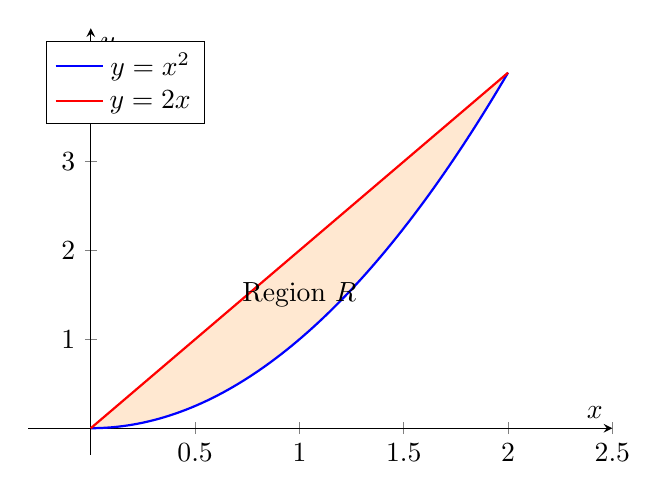
\begin{tikzpicture}
\begin{axis}[
  xlabel={$x$}, ylabel={$y$},
  xmin=-0.3, xmax=2.5, ymin=-0.3, ymax=4.5,
  axis lines=center,
  width=9cm, height=7cm,
  samples=80,
  legend pos=north west
]
\addplot[name path=A, blue, thick, domain=0:2] {x^2};
\addplot[name path=B, red, thick, domain=0:2] {2*x};
\addplot[fill=orange!30, opacity=0.6] fill between[of=A and B];
\addlegendentry{$y = x^2$}
\addlegendentry{$y = 2x$}
\node at (axis cs:1,1.5) {Region $R$};
\end{axis}
\end{tikzpicture}
\end{center}

\subsection*{Figure 2: Centroid of a Triangular Lamina}

\begin{center}
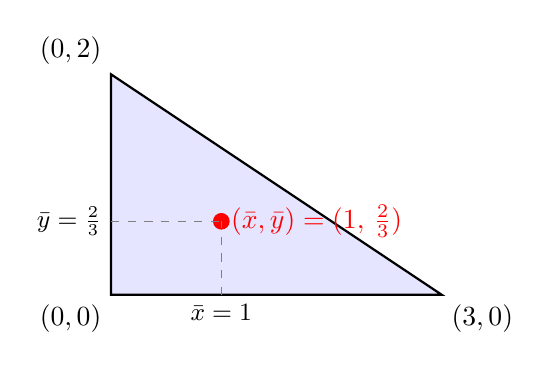
\begin{tikzpicture}[scale=1.4]
  \draw[thick, fill=blue!10] (0,0) -- (3,0) -- (0,2) -- cycle;
  \node[below left] at (0,0) {$(0,0)$};
  \node[below right] at (3,0) {$(3,0)$};
  \node[above left] at (0,2) {$(0,2)$};
  \filldraw[red] (1,0.667) circle (2pt) node[right] {$(\bar{x}, \bar{y}) = (1,\,\tfrac{2}{3})$};
  \draw[dashed, gray] (1,0) -- (1,0.667);
  \draw[dashed, gray] (0,0.667) -- (1,0.667);
  \node[below] at (1,0) {\small $\bar{x}=1$};
  \node[left] at (0,0.667) {\small $\bar{y}=\tfrac{2}{3}$};
\end{tikzpicture}
\end{center}

\subsection*{Figure 3: Moment of Inertia --- Mass Elements at Distance from Axis}

\begin{center}
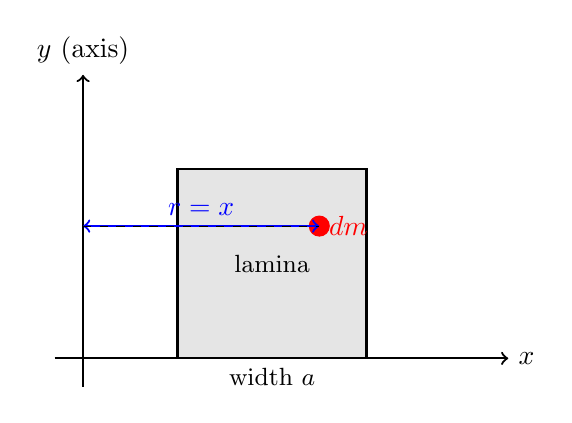
\begin{tikzpicture}[scale=1.2]
  \draw[thick, ->] (-0.3,0) -- (4.5,0) node[right] {$x$};
  \draw[thick, ->] (0,-0.3) -- (0,3.0) node[above] {$y$ (axis)};
  \draw[thick, fill=gray!20] (1,0) rectangle (3,2);
  \filldraw[red] (2.5,1.4) circle (3pt) node[right] {$dm$};
  \draw[<->, thick, blue] (0,1.4) -- (2.5,1.4) node[midway, above] {$r = x$};
  \node at (2,1) {\small lamina};
  \node[below] at (2,0) {\small width $a$};
  \draw[dashed] (0,1.4) -- (2.5,1.4);
\end{tikzpicture}
\end{center}

\subsection*{Figure 4: Volume Under a Surface \(z = 4 - x^2 - y^2\) over the Unit Square}

\begin{center}
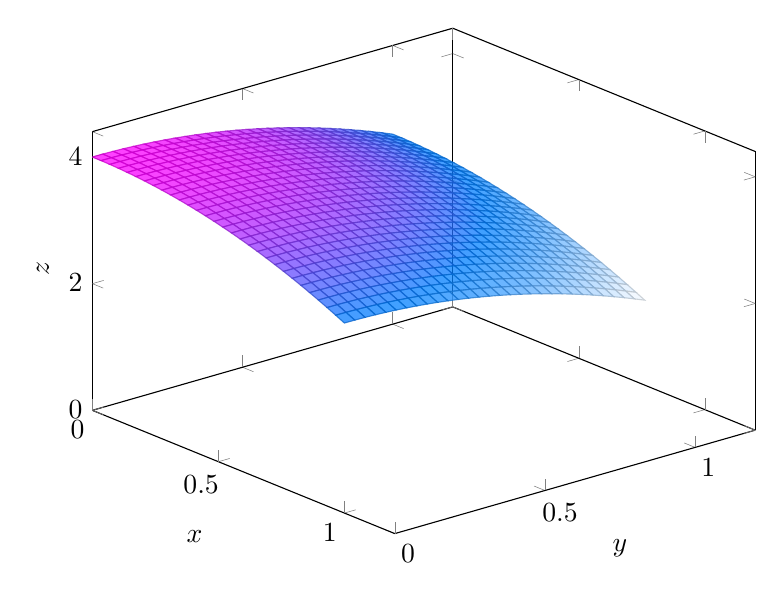
\begin{tikzpicture}
\begin{axis}[
  xlabel={$x$}, ylabel={$y$}, zlabel={$z$},
  xmin=0, xmax=1.2, ymin=0, ymax=1.2, zmin=0,
  width=10cm, height=8cm,
  view={50}{30},
  colormap/cool,
  samples=30
]
\addplot3[surf, opacity=0.75, domain=0:1, y domain=0:1]
  {4 - x^2 - y^2};
\end{axis}
\end{tikzpicture}
\end{center}

%=============================================================
\section{Step-by-Step Algorithmic Workflow}
%=============================================================

\begin{infobox}{Workflow: Setting Up and Evaluating a Multiple Integral}
\begin{enumerate}[label=\textbf{Step \arabic*.}]
  \item \textbf{Identify the physical quantity.}
        Determine whether you need area, volume, mass, centroid, moment of inertia, fluid force, charge, or probability. Each has a prescribed integrand.
  \item \textbf{Choose the correct integrand.}
        \begin{itemize}
          \item Area or volume of solid: integrand \(= 1\)
          \item Volume under surface: integrand \(= f(x,y)\)
          \item Mass: integrand \(= \rho(x,y)\)
          \item First moment \(M_y\): integrand \(= x\,\rho(x,y)\); moment \(M_x\): integrand \(= y\,\rho(x,y)\)
          \item \(I_y\): integrand \(= x^2\,\rho(x,y)\); \(I_x\): integrand \(= y^2\,\rho(x,y)\)
          \item Fluid force: integrand \(= \rho_w\,g\,h(x,y)\)
          \item Charge: integrand \(= \sigma(x,y)\)
        \end{itemize}
  \item \textbf{Determine and sketch the region \(R\).}
        Identify the boundary curves and find intersection points. Choose Cartesian or polar/cylindrical coordinates based on the shape of \(R\).
  \item \textbf{Set up the limits of integration.}
        For a Type I (vertically simple) region: outer limits on \(x\), inner limits on \(y\) as functions of \(x\). Check which boundary is upper and which is lower.
  \item \textbf{Evaluate inner integral first, then outer.}
        Treat the inner variable as the variable of integration; keep the outer variable constant. After the inner integral is done, substitute and integrate over the outer variable.
  \item \textbf{Interpret the result with correct physical units.}
        Area in m\(^2\), volume in m\(^3\), mass in kg, moment in kg\(\cdot\)m, moment of inertia in kg\(\cdot\)m\(^2\), force in N, charge in C.
\end{enumerate}
\end{infobox}

%=============================================================
\section{Fully Worked Step-by-Step Numerical Examples}
%=============================================================

\subsection*{Example 1 --- Area Between Curves}

\textbf{Problem:} Find the area enclosed between \(y = x^2\) and \(y = x + 2\).

\textit{Step 1 --- Find intersection points.}
\(x^2 = x + 2 \Rightarrow x^2 - x - 2 = 0 \Rightarrow (x-2)(x+1) = 0\). So \(x = -1\) and \(x = 2\).

\textit{Step 2 --- Identify upper curve.}
At \(x = 0\): \(y = 0 + 2 = 2 > 0 = 0^2\). Upper curve: \(y = x + 2\); lower: \(y = x^2\).

\textit{Step 3 --- Set up integral.}
\[
A = \int_{-1}^{2} \bigl[(x+2) - x^2\bigr]\,dx
\]

\textit{Step 4 --- Evaluate.}
\[
A = \left[\frac{x^2}{2} + 2x - \frac{x^3}{3}\right]_{-1}^{2}
\]
At \(x = 2\): \(\dfrac{4}{2} + 4 - \dfrac{8}{3} = 2 + 4 - \dfrac{8}{3} = 6 - \dfrac{8}{3} = \dfrac{18-8}{3} = \dfrac{10}{3}\).

At \(x = -1\): \(\dfrac{1}{2} + 2(-1) - \dfrac{(-1)^3}{3} = \dfrac{1}{2} - 2 + \dfrac{1}{3} = \dfrac{3}{6} - \dfrac{12}{6} + \dfrac{2}{6} = -\dfrac{7}{6}\).

\[
A = \frac{10}{3} - \left(-\frac{7}{6}\right) = \frac{10}{3} + \frac{7}{6} = \frac{20}{6} + \frac{7}{6} = \frac{27}{6} = \frac{9}{2}
\]

\begin{learnbox}{Key Insight --- Example 1}
Always find the intersection points first. The integrand is \emph{upper minus lower} curve; a sign error here gives a negative or wrong area. The enclosed area between \(y = x^2\) and \(y = x+2\) is \(\tfrac{9}{2}\) square units.
\end{learnbox}

\subsection*{Example 2 --- Centroid of a Triangular Lamina}

\textbf{Problem:} Find the centroid of the triangular lamina with vertices \((0,0)\), \((3,0)\), \((0,2)\) and uniform density \(\rho_0\).

\textit{Step 1 --- Equation of the hypotenuse.}
Line through \((3,0)\) and \((0,2)\): \(\dfrac{x}{3} + \dfrac{y}{2} = 1 \Rightarrow y = 2\left(1 - \dfrac{x}{3}\right) = 2 - \dfrac{2x}{3}\).

\textit{Step 2 --- Limits:} \(0 \leq x \leq 3\), \(0 \leq y \leq 2 - \dfrac{2x}{3}\).

\textit{Step 3 --- Mass.}
\[
M = \rho_0 \int_0^3 \int_0^{2 - 2x/3} dy\,dx
= \rho_0 \int_0^3 \left(2 - \frac{2x}{3}\right) dx
= \rho_0 \left[2x - \frac{x^2}{3}\right]_0^3
= \rho_0 \left(6 - 3\right) = 3\rho_0
\]
(Consistent with triangle area \(\tfrac{1}{2}\times3\times2=3\).)

\textit{Step 4 --- Moment \(M_y\).}
\[
M_y = \rho_0 \int_0^3 x\left(2 - \frac{2x}{3}\right) dx
= \rho_0 \int_0^3 \left(2x - \frac{2x^2}{3}\right) dx
= \rho_0 \left[x^2 - \frac{2x^3}{9}\right]_0^3
= \rho_0\!\left(9 - 6\right) = 3\rho_0
\]

\textit{Step 5 --- Moment \(M_x\).}
\[
M_x = \rho_0 \int_0^3 \int_0^{2-2x/3} y\,dy\,dx
= \rho_0 \int_0^3 \frac{1}{2}\left(2 - \frac{2x}{3}\right)^2 dx
\]
Let \(u = 2 - \tfrac{2x}{3}\), so \(\left(2-\tfrac{2x}{3}\right)^2 = \tfrac{4}{9}(3-x)^2\).
\[
M_x = \frac{\rho_0}{2} \int_0^3 \frac{4}{9}(3-x)^2\,dx
= \frac{2\rho_0}{9} \left[-\frac{(3-x)^3}{3}\right]_0^3
= \frac{2\rho_0}{9} \cdot \frac{27}{3}
= \frac{2\rho_0}{9} \cdot 9 = 2\rho_0
\]

\textit{Step 6 --- Centroid.}
\[
\bar{x} = \frac{M_y}{M} = \frac{3\rho_0}{3\rho_0} = 1, \qquad
\bar{y} = \frac{M_x}{M} = \frac{2\rho_0}{3\rho_0} = \frac{2}{3}
\]

\begin{learnbox}{Key Insight --- Example 2}
For a uniform triangle with vertices \((x_1,y_1)\), \((x_2,y_2)\), \((x_3,y_3)\), the centroid is always at \(\left(\tfrac{x_1+x_2+x_3}{3},\, \tfrac{y_1+y_2+y_3}{3}\right) = (1,\, \tfrac{2}{3})\) --- confirming our result.
\end{learnbox}

\subsection*{Example 3 --- Moment of Inertia (Engineering)}

\textbf{Problem:} Compute \(I_y\) for a rectangular plate \(0 \leq x \leq a\), \(0 \leq y \leq b\) with uniform density \(\rho_0\). Find the radius of gyration \(k_y\) and explain its significance for beam design.

\textit{Step 1 --- Moment of inertia \(I_y\).}
\[
I_y = \int_0^a \int_0^b x^2\,\rho_0\,dy\,dx
= \rho_0 \int_0^a x^2 [y]_0^b\,dx
= \rho_0 b \int_0^a x^2\,dx
= \rho_0 b \left[\frac{x^3}{3}\right]_0^a
= \frac{\rho_0\, a^3 b}{3}
\]

\textit{Step 2 --- Total mass.}
\[
M = \rho_0 \cdot a \cdot b
\]

\textit{Step 3 --- Radius of gyration.}
\[
k_y = \sqrt{\frac{I_y}{M}} = \sqrt{\frac{\rho_0 a^3 b / 3}{\rho_0 ab}} = \sqrt{\frac{a^2}{3}} = \frac{a}{\sqrt{3}}
\]

\textit{Step 4 --- Engineering interpretation.}
For \(a = 0.3\,\text{m}\), \(b = 0.1\,\text{m}\), \(\rho_0 = 7800\,\text{kg/m}^2\) (steel plate):
\[
I_y = \frac{7800 \times (0.3)^3 \times 0.1}{3} = \frac{7800 \times 0.027 \times 0.1}{3} = \frac{21.06}{3} = 7.02\,\text{kg\,m}^2
\]
\[
k_y = \frac{0.3}{\sqrt{3}} \approx 0.1732\,\text{m}
\]
A structural engineer uses \(I_y\) to check the beam's resistance to bending about the \(y\)-axis; a larger \(I_y\) means greater stiffness.

\begin{learnbox}{Key Insight --- Example 3}
\(I_y = \tfrac{\rho_0 a^3 b}{3}\) grows as \(a^3\), so doubling the width \(a\) increases bending stiffness eightfold. The radius of gyration \(k_y = a/\sqrt{3}\) is the equivalent arm at which the total mass would produce the same \(I_y\).
\end{learnbox}

\subsection*{Example 4 --- Fluid Pressure on a Triangular Dam Gate (Mandatory)}

\textbf{Problem:} A triangular dam gate is submerged vertically in water. The gate has vertices at \((0,0)\), \((2,0)\), and \((1,3)\) in the \(xy\)-plane, where \(y\) measures depth below the water surface (in metres). Compute the total fluid pressure force on the gate using \(F = \iint_R \rho_w\,g\,h(x,y)\,dA\), where \(\rho_w = 1000\,\text{kg/m}^3\), \(g = 9.81\,\text{m/s}^2\), and \(h(x,y) = y\) (depth equals \(y\)-coordinate).

\textit{Step 1 --- Describe the region \(R\).}
The three edges of the triangle are:
\begin{itemize}
  \item Bottom edge: \(y = 0\), from \(x = 0\) to \(x = 2\).
  \item Left edge: from \((0,0)\) to \((1,3)\). Slope \(= 3\), equation \(x = y/3\).
  \item Right edge: from \((2,0)\) to \((1,3)\). Slope \(= (3-0)/(1-2) = -3\), equation \(x = 2 - y/3\).
\end{itemize}

For a fixed \(y\) (\(0 \leq y \leq 3\)), \(x\) ranges from \(y/3\) to \(2 - y/3\).

\textit{Step 2 --- Set up the integral.}
\[
F = \rho_w\,g \int_0^3 \int_{y/3}^{2-y/3} y\,dx\,dy
\]

\textit{Step 3 --- Evaluate the inner integral.}
\[
\int_{y/3}^{2-y/3} y\,dx = y \cdot \left[(2 - y/3) - y/3\right] = y\!\left(2 - \frac{2y}{3}\right) = 2y - \frac{2y^2}{3}
\]

\textit{Step 4 --- Evaluate the outer integral.}
\[
\int_0^3 \left(2y - \frac{2y^2}{3}\right) dy
= \left[y^2 - \frac{2y^3}{9}\right]_0^3
= \left(9 - \frac{2 \times 27}{9}\right)
= 9 - 6 = 3
\]

\textit{Step 5 --- Compute the force.}
\[
F = \rho_w\,g \times 3 = 1000 \times 9.81 \times 3 = 29430\,\text{N} \approx 29.43\,\text{kN}
\]

\begin{learnbox}{Key Insight --- Example 4}
The hydrostatic pressure \(\rho_w g y\) varies linearly with depth. Integrating it over the gate area gives the total force; simply multiplying by gate area would be wrong because pressure is not uniform. The total force on this 3~m tall triangular gate is approximately \(29.43\,\text{kN}\).
\end{learnbox}

%=============================================================
\section{Tabular Reference and Workflow Summary}
%=============================================================

\begin{center}
\small
\begin{tabular}{>{\bfseries}p{3.5cm} p{4.5cm} p{2.5cm} p{3cm}}
\toprule
Physical Quantity & Formula & Integrand & Notes on Units \\
\midrule
Area of region \(R\) &
\(A = \iint_R dA\) & \(1\) & m\(^2\) \\[4pt]
Volume under surface &
\(V = \iint_R f(x,y)\,dA\) & \(f(x,y)\) & m\(^3\) \\[4pt]
Volume of solid \(E\) &
\(V = \iiint_E dV\) & \(1\) & m\(^3\) \\[4pt]
Mass (2D) &
\(M = \iint_R \rho(x,y)\,dA\) & \(\rho(x,y)\) & kg \\[4pt]
Mass (3D) &
\(M = \iiint_E \rho\,dV\) & \(\rho(x,y,z)\) & kg \\[4pt]
Centroid \(\bar{x}\) &
\(\bar{x} = M_y/M\) &
\(x\,\rho(x,y)\) & m \\[4pt]
Centroid \(\bar{y}\) &
\(\bar{y} = M_x/M\) &
\(y\,\rho(x,y)\) & m \\[4pt]
\(I_x\) (about \(x\)-axis) &
\(I_x = \iint_R y^2\rho\,dA\) & \(y^2\rho\) & kg\,m\(^2\) \\[4pt]
\(I_y\) (about \(y\)-axis) &
\(I_y = \iint_R x^2\rho\,dA\) & \(x^2\rho\) & kg\,m\(^2\) \\[4pt]
\(I_0\) (polar / \(z\)-axis) &
\(I_0 = I_x + I_y\) & \((x^2+y^2)\rho\) & kg\,m\(^2\) \\[4pt]
Radius of gyration &
\(k = \sqrt{I/M}\) & --- & m \\[4pt]
Fluid pressure force &
\(F = \iint_R \rho_w g h\,dA\) & \(\rho_w g h(x,y)\) & N \\[4pt]
Electric charge &
\(Q = \iint_R \sigma\,dA\) & \(\sigma(x,y)\) & C \\
\bottomrule
\end{tabular}
\end{center}

%=============================================================
\section{Common Student Mistakes and Pitfalls}
%=============================================================

\begin{mistakebox}{Common Mistakes in Applications of Multiple Integration}
\begin{tabular}{>{\bfseries}p{4cm} p{4.5cm} p{5cm}}
\toprule
Mistake & Why It Is Wrong & Correct Approach \\
\midrule
Using integrand \(1\) for mass instead of \(\rho(x,y)\) &
Mass \(\neq\) area; density weights each area element &
Always write \(M = \iint_R \rho(x,y)\,dA\); substitute \(\rho\) before integrating \\[6pt]
Confusing \(M_x\) with \(\bar{x}\) &
\(M_x = \iint_R y\rho\,dA\) is a moment about the \(x\)-axis, not the centroid \(x\)-coordinate &
Centroid: \(\bar{x} = M_y/M\) and \(\bar{y} = M_x/M\); subscripts on moments and coordinates refer to different axes \\[6pt]
Using \(r = \sqrt{x^2+y^2}\) (distance from origin) for \(I_x\) or \(I_y\) &
Moment of inertia about the \(x\)-axis uses \(r = y\) (perpendicular distance from \(x\)-axis), not distance from origin &
\(I_x = \iint y^2\rho\,dA\); \(I_y = \iint x^2\rho\,dA\); polar moment \(I_0\) uses \(r^2 = x^2+y^2\) \\[6pt]
Multiplying pressure by area for fluid force &
Pressure \(\rho_w g h\) varies with depth; multiplying average pressure by area is valid only for rectangular gates with depth measured to centroid &
Use \(F = \iint_R \rho_w g h(x,y)\,dA\) and integrate over the actual gate region \\[6pt]
Swapping limits of integration &
Writing outer limits as functions of the inner variable violates the definition of iterated integrals &
Outer limits must be constants; inner limits may be functions of the outer variable only \\[6pt]
Forgetting Jacobian in polar coordinates &
Converting \(dA = dx\,dy\) to polar without the factor \(r\) gives a wrong result by a factor of \(r\) &
In polar: \(dA = r\,dr\,d\theta\); always include the \(r\) Jacobian factor \\
\bottomrule
\end{tabular}
\end{mistakebox}

%=============================================================
\section{Comprehensive Assessment Suite}
%=============================================================

\subsection*{Viva-Voce Questions}

\begin{enumerate}[label=\textbf{V\arabic*.}]

  \item \textbf{(Area and Volume)} How do you decide whether to use a double integral or a triple integral to compute the volume of a given solid? Explain with reference to the geometry of the problem. \\
  \textit{Hint:} If the solid is described as a region below a surface \(z = f(x,y)\) over a 2D region \(R\), use \(\iint_R f(x,y)\,dA\). If the solid is defined by inequalities in all three variables, use \(\iiint_E dV\).

  \item \textbf{(Area and Volume)} Explain why the area formula \(A = \iint_R dA\) is a special case of the volume formula \(V = \iint_R f(x,y)\,dA\). \\
  \textit{Hint:} Setting \(f(x,y) = 1\) gives a surface of unit height; the volume of a unit-height slab equals the base area.

  \item \textbf{(Mass and Centroid)} What is the physical meaning of the centroid of a lamina, and why does it coincide with the geometric centre only when the density is uniform? \\
  \textit{Hint:} The centroid is the balance point; non-uniform density shifts it toward the denser region.

  \item \textbf{(Mass and Centroid)} Define the first moments \(M_x\) and \(M_y\) of a lamina. Which moment is used to compute \(\bar{x}\) and which is used to compute \(\bar{y}\)? \\
  \textit{Hint:} \(\bar{x} = M_y/M\) and \(\bar{y} = M_x/M\). The subscripts indicate the axis about which the moment is taken.

  \item \textbf{(Moment of Inertia)} Why does the moment of inertia of a rotating object increase when mass is shifted farther from the rotation axis? Relate your answer to the formula \(I = \iint r^2\,\rho\,dA\). \\
  \textit{Hint:} The \(r^2\) factor means contributions grow quadratically with distance, making remote mass much more influential than nearby mass.

  \item \textbf{(Moment of Inertia)} What is the radius of gyration \(k\), and how does it help a structural engineer compare two beams of the same mass? \\
  \textit{Hint:} \(k = \sqrt{I/M}\); a larger \(k\) indicates that the mass is distributed farther from the axis, meaning greater bending stiffness for the same total mass.

  \item \textbf{(Engineering Applications)} Set up the double integral for the total hydrostatic force on a rectangular gate of width \(w\) and height \(H\) submerged vertically with its top edge at depth \(d\) below the water surface. \\
  \textit{Hint:} \(h(x,y) = d + y\) if \(y\) is measured downward from the top of the gate; \(F = \rho_w g \int_0^w \int_0^H (d+y)\,dy\,dx\).

  \item \textbf{(Engineering Applications)} How is the formula \(P = \iint_R f(x,y)\,dA\) for probability analogous to the formula for mass, and what constraint must \(f(x,y)\) satisfy for it to be a valid joint probability density function? \\
  \textit{Hint:} \(f(x,y) \geq 0\) everywhere and \(\iint_{\mathbb{R}^2} f(x,y)\,dA = 1\); \(f\) plays the role of density and the integral over any region gives the probability for that region.

\end{enumerate}

\subsection*{Descriptive Exam Questions}

\begin{enumerate}[label=\textbf{D\arabic*.}]

  \item Find the area of the region bounded by the parabola \(y = x^2 - 4\) and the line \(y = 2x - 1\). Show the intersection points and write the double integral in full before evaluating. \\
  \textit{Answer hint:} Intersections at \(x = 3\) and \(x = -1\); upper curve is \(y = 2x-1\); area \(= \int_{-1}^{3}[(2x-1)-(x^2-4)]\,dx = \tfrac{32}{3}\).

  \item A lamina occupies the region \(0 \leq x \leq 2\), \(0 \leq y \leq 3\) with density \(\rho(x,y) = 2x + y\). Find the total mass, the moments \(M_x\) and \(M_y\), and the centroid. Show every integration step. \\
  \textit{Answer hint:} \(M = 18\); \(M_y = 16\); \(M_x = 27\); \(\bar{x} = 8/9\); \(\bar{y} = 3/2\).

  \item Compute the polar moment of inertia \(I_0\) for the circular disc \(x^2 + y^2 \leq R^2\) with uniform surface density \(\rho_0\). Use polar coordinates. Show the Jacobian and all steps. \\
  \textit{Answer hint:} \(I_0 = \int_0^{2\pi}\int_0^R r^2 \rho_0 r\,dr\,d\theta = \tfrac{\pi\rho_0 R^4}{2}\).

  \item A rectangular channel gate is 4~m wide and 5~m tall. Its top edge is at 1~m below the water surface. Set up and evaluate the double integral for the total hydrostatic force on the gate. Express the answer in kN. \\
  \textit{Answer hint:} \(F = \rho_w g \int_0^4\int_0^5(1+y)\,dy\,dx = 1000 \times 9.81 \times 4\times(5 + 12.5) = 686.7\,\text{kN}\).

  \item The joint probability density of two random variables is \(f(x,y) = c(x+y)\) on \(0 \leq x \leq 1\), \(0 \leq y \leq 1\) and zero otherwise. (a) Find \(c\). (b) Find \(P(X + Y \leq 1)\). \\
  \textit{Answer hint:} (a) \(\iint f\,dA = c \cdot 1 = 1 \Rightarrow c = 1\). (b) Integrate over triangle \(x+y \leq 1\): \(P = \int_0^1\int_0^{1-x}(x+y)\,dy\,dx = 1/3\).

\end{enumerate}

\subsection*{Multiple Choice Questions}

\begin{enumerate}[label=\textbf{MCQ\arabic*.}]

  \item \textbf{(Area and Volume)} The area of the region bounded by \(y = x^2\) and \(y = 4\) is:
  \begin{enumerate}[label=(\alph*)]
    \item \(\dfrac{32}{3}\) \quad \textbf{(b) \(\dfrac{32}{3}\)} \quad (Wait --- options below)
  \end{enumerate}
  \begin{enumerate}[label=(\alph*)]
    \item \(8\)
    \item \(\dfrac{16}{3}\)
    \item \(\textbf{\(\dfrac{32}{3}\)}\)
    \item \(16\)
  \end{enumerate}
  \textit{Correct answer: (c).} Intersection at \(x = \pm2\); \(A = \int_{-2}^{2}(4-x^2)\,dx = [4x - x^3/3]_{-2}^{2} = 32/3\).

  \item \textbf{(Mass and Centroid)} The centroid \(\bar{y}\) of a uniform semicircular lamina of radius \(R\) (flat edge on the \(x\)-axis) is:
  \begin{enumerate}[label=(\alph*)]
    \item \(\dfrac{R}{2}\)
    \item \(\dfrac{4R}{3\pi}\)  \quad \(\leftarrow\) \textbf{correct}
    \item \(\dfrac{R}{\pi}\)
    \item \(\dfrac{2R}{3}\)
  \end{enumerate}
  \textit{Correct answer: (b) \(\mathbf{4R/(3\pi)}\).} This is the standard result from integrating in polar coordinates: \(\bar{y} = \tfrac{4R}{3\pi}\).

  \item \textbf{(Moment of Inertia)} For a square plate of side \(a\) and uniform density \(\rho_0\) with one corner at the origin, \(I_y = \):
  \begin{enumerate}[label=(\alph*)]
    \item \(\dfrac{\rho_0 a^3}{3}\)
    \item \(\dfrac{\rho_0 a^4}{3}\)  \quad \(\leftarrow\) \textbf{correct}
    \item \(\dfrac{\rho_0 a^4}{4}\)
    \item \(\dfrac{\rho_0 a^3}{4}\)
  \end{enumerate}
  \textit{Correct answer: (b) \(\mathbf{\rho_0 a^4/3}\).} \(I_y = \rho_0 \int_0^a\int_0^a x^2\,dy\,dx = \rho_0 a \cdot [x^3/3]_0^a = \rho_0 a^4/3\).

  \item \textbf{(Engineering Applications)} A flat horizontal plate of area \(A\) is submerged at uniform depth \(d\). The total hydrostatic force on it is:
  \begin{enumerate}[label=(\alph*)]
    \item \(\rho_w g A^2 d\)
    \item \(\rho_w g d / A\)
    \item \(\textbf{\(\rho_w g d A\)}\)
    \item \(\rho_w g d^2 A\)
  \end{enumerate}
  \textit{Correct answer: (c) \(\mathbf{\rho_w g d A}\).} Since depth \(h = d\) is constant, \(F = \iint_R \rho_w g d\,dA = \rho_w g d A\).

  \item \textbf{(Moment of Inertia)} The radius of gyration of a body with moment of inertia \(I = 50\,\text{kg\,m}^2\) and mass \(M = 200\,\text{kg}\) is:
  \begin{enumerate}[label=(\alph*)]
    \item \(4\,\text{m}\)
    \item \(0.5\,\text{m}\)  \quad \(\leftarrow\) \textbf{correct}
    \item \(2\,\text{m}\)
    \item \(0.25\,\text{m}\)
  \end{enumerate}
  \textit{Correct answer: (b) \(\mathbf{0.5\,\text{m}}\).} \(k = \sqrt{I/M} = \sqrt{50/200} = \sqrt{0.25} = 0.5\,\text{m}\).

  \item \textbf{(Area and Volume)} Which of the following correctly represents the volume of the solid bounded above by \(z = 1 - x - y\) and below by \(z = 0\) over the region \(R: x \geq 0, y \geq 0, x+y \leq 1\)?
  \begin{enumerate}[label=(\alph*)]
    \item \(\int_0^1\int_0^1 (1-x-y)\,dy\,dx\)
    \item \(\int_0^1\int_0^{1-x}(1-x-y)\,dy\,dx\)  \quad \(\leftarrow\) \textbf{correct}
    \item \(\int_0^1\int_0^{x}(1-x-y)\,dy\,dx\)
    \item \(\int_0^1\int_x^1 (1-x-y)\,dy\,dx\)
  \end{enumerate}
  \textit{Correct answer: (b).} For fixed \(x\), \(y\) ranges from \(0\) to \(1-x\) inside the triangle \(x+y \leq 1\).

\end{enumerate}

%=============================================================
\section{Quick Recap and Formula Sheet}
%=============================================================

\begin{learnbox}{Formula Sheet --- Applications of Multiple Integration}
\begin{itemize}[leftmargin=1.5em]
  \item \textbf{Area:} \(A = \iint_R dA\); between curves: \(A = \int_a^b [g_2(x) - g_1(x)]\,dx\).
  \item \textbf{Volume:} Under surface: \(V = \iint_R f(x,y)\,dA\); solid: \(V = \iiint_E dV\).
  \item \textbf{Mass and centroid (2D):} \(M = \iint_R \rho\,dA\); \(\bar{x} = M_y/M = \tfrac{1}{M}\iint_R x\rho\,dA\); \(\bar{y} = M_x/M = \tfrac{1}{M}\iint_R y\rho\,dA\).
  \item \textbf{Moment of inertia:} \(I_x = \iint_R y^2\rho\,dA\); \(I_y = \iint_R x^2\rho\,dA\); polar: \(I_0 = I_x + I_y\).
  \item \textbf{Radius of gyration:} \(k_x = \sqrt{I_x/M}\); \(k_y = \sqrt{I_y/M}\); \(k_0 = \sqrt{I_0/M}\).
  \item \textbf{Fluid pressure force:} \(F = \iint_R \rho_w g h(x,y)\,dA\); depth \(h(x,y)\) is the perpendicular distance below the free surface.
  \item \textbf{Electric charge:} \(Q = \iint_R \sigma(x,y)\,dA\); in polar: include Jacobian \(r\).
  \item \textbf{Polar coordinate reminder:} \(dA = r\,dr\,d\theta\); always include the factor \(r\) when changing variables.
\end{itemize}
\end{learnbox}

\end{document}
